
\subsection{UniSiegen}

This dataset is made available in 2014 by the University of Siegen, Germany.
It was constructed by dr. D. Zukic \cite{Zukic2014} as part of his PhD project.

\marginpar{
        % This file was created by tikzplotlib v0.9.8.
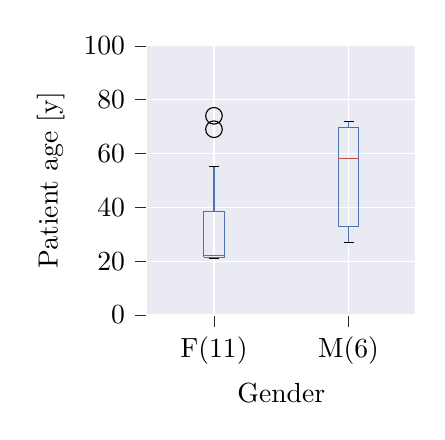
\begin{tikzpicture}

\definecolor{color0}{rgb}{0.917647058823529,0.917647058823529,0.949019607843137}
\definecolor{color1}{rgb}{0.298039215686275,0.447058823529412,0.690196078431373}
\definecolor{color2}{rgb}{0.768627450980392,0.305882352941176,0.32156862745098}

\begin{axis}[
axis background/.style={fill=color0},
axis line style={white},
height=5cm,
tick align=outside,
tick pos=left,
width=5cm,
x grid style={white},
xlabel={Gender},
xmajorgrids,
xmin=0.5, xmax=2.5,
xtick style={color=white!15!black},
xtick={1,2},
xticklabels={F(11),M(6)},
y grid style={white},
ylabel={Patient age [y]},
ymajorgrids,
ymin=0, ymax=100,
ytick style={color=white!15!black}
]
\addplot [color1, opacity=1]
table {%
0.925 21.5
1.075 21.5
1.075 38.5
0.925 38.5
0.925 21.5
};
\addplot [color1, opacity=1]
table {%
1 21.5
1 21
};
\addplot [color1, opacity=1]
table {%
1 38.5
1 55
};
\addplot [black, opacity=1]
table {%
0.9625 21
1.0375 21
};
\addplot [black, opacity=1]
table {%
0.9625 55
1.0375 55
};
\addplot [black, mark=o, mark size=3, mark options={solid,fill opacity=0}, only marks]
table {%
1 74
1 69
};
\addplot [color1, opacity=1]
table {%
1.925 33
2.075 33
2.075 69.5
1.925 69.5
1.925 33
};
\addplot [color1, opacity=1]
table {%
2 33
2 27
};
\addplot [color1, opacity=1]
table {%
2 69.5
2 72
};
\addplot [black, opacity=1]
table {%
1.9625 27
2.0375 27
};
\addplot [black, opacity=1]
table {%
1.9625 72
2.0375 72
};
\addplot [color2, opacity=1]
table {%
0.925 22
1.075 22
};
\addplot [color2, opacity=1]
table {%
1.925 58
2.075 58
};
\end{axis}

\end{tikzpicture}

        \captionof{figure}{USiegen patients age distribution}
        \label{fig:USiegen_Age}
    }

This dataset contains 26 \acrshort{mri} scans of 17 different patients. 
The fact that scans of the same patient are correlated will be taken into account 

\subsubsection{Original Objective of the Dataset}

This dataset was collected from several hospitals (Sarajevo, Marburg, Brisbane, Schwabach, Bad Wildungen \& Prague). The MRI scanner settings were varied between the scans (T1, T2, TIRM).
The PhD project objective was to build a segmentation model to automate the segmentation of the lumbar vertebrae in the \acrshort{mri} scans to facilitate the diagnosis of several spine pathologies 
such as scoliosis, spondylolisthesis \footnote{Spondylolisthesis is the displacement of one spinal vertebra compared to another.} and vertebral fractures.
The final model developed by dr. D. Zukic consisted of a Viola-Jones detector for detection and vertebral body size approximation.
The average Dice score compared to the manual reference was reported to be 79.3\%.

\subsubsection{Patient statistics}

Figure \ref{fig:USiegen_Age} illustrates that the USiegen dataset contains almost double the amount of female patients compared to male patients.
These patients are relatively young compared to the patients in the \textit{xVertSeg} dataset.

\begin{SCfigure}[][htb]
    \centering
    \begin{minipage}{.5\textwidth}
        % This file was created by tikzplotlib v0.9.8.
\begin{tikzpicture}

\definecolor{color0}{rgb}{0.917647058823529,0.917647058823529,0.949019607843137}

\begin{axis}[
axis background/.style={fill=color0},
axis line style={white},
height=5cm,
tick align=outside,
tick pos=left,
width=5cm,
x grid style={white},
xlabel={Anteroposterior axis (x) [mm]},
xmin=-0.5, xmax=359.5,
xtick style={color=white!15!black},
y dir=reverse,
y grid style={white},
ylabel={Craniocaudal axis (y) [mm]},
ymin=-0.5, ymax=359.5,
ytick style={color=white!15!black}
]
\addplot graphics [includegraphics cmd=\pgfimage,xmin=-0.5, xmax=359.5, ymin=359.5, ymax=-0.5] {USiegen_Aka3_SagitalSlice-000.png};
\end{axis}

\end{tikzpicture}

    \end{minipage}%
    \begin{minipage}{0.5\textwidth}
        % This file was created by tikzplotlib v0.9.8.
\begin{tikzpicture}

\definecolor{color0}{rgb}{0.917647058823529,0.917647058823529,0.949019607843137}

\begin{axis}[
axis background/.style={fill=color0},
axis line style={white},
height=3cm,
tick align=outside,
tick pos=left,
width=5cm,
x grid style={white},
xlabel={Anteroposterior axis (x) [mm]},
xmin=-0.5, xmax=359.5,
xtick style={color=white!15!black},
y dir=reverse,
y grid style={white},
ylabel={Left-right axis (z) [mm]},
ymin=-0.5, ymax=59.5,
ytick style={color=white!15!black}
]
\addplot graphics [includegraphics cmd=\pgfimage,xmin=-0.5, xmax=359.5, ymin=59.5, ymax=-0.5] {automated_graphs/USiegen_Aka3_TransversalSlice-000.png};
\end{axis}

\end{tikzpicture}

    \end{minipage}
    \caption{Scan \textit{Aka3} of the USiegen dataset. Sagittal slice on the left and Transverse slice on the right.\label{fig:xVertSeg_image002}}
\end{SCfigure}

The scans were cropped in the \textit{left-right} direction. 

\begin{SCfigure}[][htb]
    \centering
    % This file was created by tikzplotlib v0.9.8.
\begin{tikzpicture}

\definecolor{color0}{rgb}{0,0.447058823529412,0.698039215686274}
\definecolor{color1}{rgb}{0.835294117647059,0.368627450980392,0}

\begin{groupplot}[group style={group size=1 by 2}]
\nextgroupplot[
height=7cm,
tick align=outside,
tick pos=left,
width=9cm,
x grid style={white!69.0196078431373!black},
xmin=0.5, xmax=3.5,
xtick style={color=black},
y grid style={white!69.0196078431373!black},
ylabel={dimension [mm]},
ymin=30.439999296, ymax=522.360014784,
ytick style={color=black},
ytick={0,100,200,300,400,500,600},
yticklabels={0,200,400,600,,,}
]
\addplot [color0, opacity=1]
table {%
1 352
1 350
};
\addplot [color0, opacity=1]
table {%
1 359.9872
1 359.9872
};
\addplot [black, opacity=1]
table {%
0.925 350
1.075 350
};
\addplot [black, opacity=1]
table {%
0.925 359.9872
1.075 359.9872
};
\addplot [black, mark=o, mark size=3, mark options={solid,fill opacity=0}, only marks]
table {%
1 300.85470208
1 300.85470208
1 380
1 500.00001408
1 500.00001408
1 380.540542464
};
\addplot [color0, opacity=1]
table {%
2 352
2 350
};
\addplot [color0, opacity=1]
table {%
2 359.9872
2 359.9872
};
\addplot [black, opacity=1]
table {%
1.925 350
2.075 350
};
\addplot [black, opacity=1]
table {%
1.925 359.9872
2.075 359.9872
};
\addplot [black, mark=o, mark size=3, mark options={solid,fill opacity=0}, only marks]
table {%
2 300.85470208
2 300.85470208
2 380
2 500.00001408
2 500.00001408
2 380.540542464
};
\addplot [color0, opacity=1]
table {%
3 60
3 52.8
};
\addplot [color0, opacity=1]
table {%
3 69.30001998
3 82.5000115
};
\addplot [black, opacity=1]
table {%
2.925 52.8
3.075 52.8
};
\addplot [black, opacity=1]
table {%
2.925 82.5000115
3.075 82.5000115
};
\addplot [black, mark=o, mark size=3, mark options={solid,fill opacity=0}, only marks]
table {%
3 102.3000031
3 100
};
\path [draw=color0, fill=color0]
(axis cs:0.85,352)
--(axis cs:1.15,352)
--(axis cs:1.15,359.9872)
--(axis cs:0.85,359.9872)
--(axis cs:0.85,352)
--cycle;
\path [draw=color0, fill=color0]
(axis cs:1.85,352)
--(axis cs:2.15,352)
--(axis cs:2.15,359.9872)
--(axis cs:1.85,359.9872)
--(axis cs:1.85,352)
--cycle;
\path [draw=color0, fill=color0]
(axis cs:2.85,60)
--(axis cs:3.15,60)
--(axis cs:3.15,69.30001998)
--(axis cs:2.85,69.30001998)
--(axis cs:2.85,60)
--cycle;
\addplot [color1, opacity=1]
table {%
0.85 359.9872
1.15 359.9872
};
\addplot [color1, opacity=1]
table {%
1.85 359.9872
2.15 359.9872
};
\addplot [color1, opacity=1]
table {%
2.85 60
3.15 60
};

\nextgroupplot[
height=7cm,
tick align=outside,
tick pos=left,
width=9cm,
x grid style={white!69.0196078431373!black},
xmin=0.5, xmax=3.5,
xtick style={color=black},
xtick={1,2,3},
xticklabels={anteroposterior (x),craniocaudal (y),left-right (z)},
y grid style={white!69.0196078431373!black},
ylabel={spacing [mm]},
ymin=0.2735897456, ymax=4.5964957264,
ytick style={color=black},
ytick={0,1,2,3,4,5},
yticklabels={0,2,4,6,,}
]
\addplot [color0, opacity=1]
table {%
1 0.546875
1 0.470085472
};
\addplot [color0, opacity=1]
table {%
1 0.7031
1 0.7031
};
\addplot [black, opacity=1]
table {%
0.925 0.470085472
1.075 0.470085472
};
\addplot [black, opacity=1]
table {%
0.925 0.7031
1.075 0.7031
};
\addplot [black, mark=o, mark size=3, mark options={solid,fill opacity=0}, only marks]
table {%
1 1.1875
1 1.11607146
1 1.11607146
};
\addplot [color0, opacity=1]
table {%
2 0.546875
2 0.470085472
};
\addplot [color0, opacity=1]
table {%
2 0.7031
2 0.7031
};
\addplot [black, opacity=1]
table {%
1.925 0.470085472
2.075 0.470085472
};
\addplot [black, opacity=1]
table {%
1.925 0.7031
2.075 0.7031
};
\addplot [black, mark=o, mark size=3, mark options={solid,fill opacity=0}, only marks]
table {%
2 1.1875
2 1.11607146
2 1.11607146
};
\addplot [color0, opacity=1]
table {%
3 3.85000083
3 3.8499985
};
\addplot [color0, opacity=1]
table {%
3 4
3 4
};
\addplot [black, opacity=1]
table {%
2.925 3.8499985
3.075 3.8499985
};
\addplot [black, opacity=1]
table {%
2.925 4
3.075 4
};
\addplot [black, mark=o, mark size=3, mark options={solid,fill opacity=0}, only marks]
table {%
3 3.30000046
3 3.3000001
3 3.00000269
3 4.4
3 4.4
};
\path [draw=color0, fill=color0]
(axis cs:0.85,0.546875)
--(axis cs:1.15,0.546875)
--(axis cs:1.15,0.7031)
--(axis cs:0.85,0.7031)
--(axis cs:0.85,0.546875)
--cycle;
\path [draw=color0, fill=color0]
(axis cs:1.85,0.546875)
--(axis cs:2.15,0.546875)
--(axis cs:2.15,0.7031)
--(axis cs:1.85,0.7031)
--(axis cs:1.85,0.546875)
--cycle;
\path [draw=color0, fill=color0]
(axis cs:2.85,3.85000083)
--(axis cs:3.15,3.85000083)
--(axis cs:3.15,4)
--(axis cs:2.85,4)
--(axis cs:2.85,3.85000083)
--cycle;
\addplot [color1, opacity=1]
table {%
0.85 0.7031
1.15 0.7031
};
\addplot [color1, opacity=1]
table {%
1.85 0.7031
2.15 0.7031
};
\addplot [color1, opacity=1]
table {%
2.85 4
3.15 4
};
\end{groupplot}

\end{tikzpicture}

    \caption{Distribution of the dimensions of the USiegen images. \label{fig:USiegen_Dims}}
\end{SCfigure}

\subsubsection{Technical information}


